\section{Design}
\label{sec:design}

In this section we describe our design for a fully
disaggregated lock-based cuckoo hash. We first describe our
table design and protocol to read, insert, update and delete
entries from the table. Next we describe a novel locality
based hashing algorithm and how it enables our protocol to
perform most operations in two round trips or less. To close
we detail how RCuckoo detects and recovers from client
failures.



\subsection{Table Design}
\label{sec:table-design}

Figure~\ref{fig:table-diagram} shows RCuckoos index and lock
table during an insertion of key $K$. The primary row for
$K$ is full and key $C$ is evicted to its alternate
location. Locks for $K$ and $C$ are set in lock table. Here
locks protect two rows each.
%%
The table index (right) is a single region of RDMA
registered main memory with fixed width entries.  Each row
contains $n$ associative entries (3 in
Figure~\ref{fig:table-diagram}) and terminates with an 8 bit
version number and 64 bit CRC. Inlined table entries begin
with a 0 bit and directly store both key and value. Extent
entries for large values ~\footnote{Inlined entries perform
better on small key value pairs} store pointers to kv pairs
stored outside the index.
%%
When an entry is modified it's rows version number is
incremented and its CRC is recalculated including the
updated version number. CRC's enable lockless reads as each
row can be self verified. Version numbers enable clients to
detect if a row has been modified by polling CRCs which is
used to detect if a client has failed while holding a lock
(Section~\ref{sec:fault-tolerance}).

% The lock table
% (Section~\ref{sec:locking}) is shown on the left~\todo{add
% virtual table}. 
% ~\todo{We leave resizing to future work.}. 
%%
% \textbf{Client Caching:}
%%

Rcuckoo clients keep an RDMA registered cache of the index
locally. Caches can be purged or persisted between requests
depending on a clients available memory. Clients synchronize
their caches during inserts to perform local searches when
insertions require multiple retries. While theoretically
these caches could be persisted to improve performance our
experimentation shows that due to high churn in the cuckoo
index lock granularity paired with read strategy
(Section~\ref{sec:insert}) has a far higher impact on search
success over caching (Section~\ref{sec:search_success}).

% \textbf{Memory Allocation:}
% %%
% \sg{Help alex, I need to remove this section but I don't
% quite know how to talk about memory allocation or extent
% memory}
% %%
% Prior work has focused on different memory allocation and
% hash table resizing schemes. Sherman~\cite{sherman} uses an
% allocated thread located on the memory node,
% Fusee~\cite{fusee} uses a two tired memory allocation in
% which large blocks of memory are allocated on the memory
% nodes and fine grained allocation is performed on the
% clients. Clover~\cite{clover} statically partitions memory
% into large client regions prior to execution and hash
% clients entirely manage the space themselves. Network based
% allocators such as MIND and Clio~\cite{mind,clio} have
% demonstrated the feasibility of high performance
% disaggregated allocators, while some have called for
% allocators to be built into RDMA~\cite{prism}. We allocate
% memory using the same scheme as Clover, as it is simple to
% implement and adds no additional overhead. We view memory
% allocation as a hard orthogonal problem to the design of
% disaggregated indexes and have designed our system
% acrostically to the allocator.

\begin{figure}[t]
    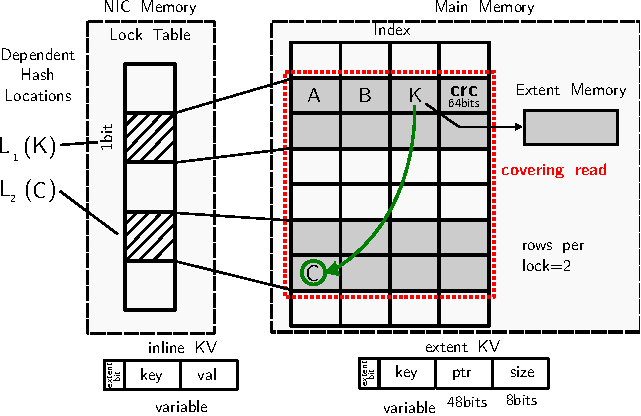
\includegraphics[width=0.99\linewidth]{fig/table-diagram.pdf}
    \caption{Rcuckoo's table design showing an insert of the key $K$ as it displaces $C$.~\todo{add lease table}}
    \label{fig:table-diagram}
\end{figure}



% In this section we describe our protocol for reading,
% inserting, and performing updates and deletes to an rcuckoo
% hash table. Figure~\ref{fig:message_diagram} visualizes our
% protocol.

\subsubsection{Reads, Updates, and Deletes} 
\label{sec:reading}

Our table is designed to facility lockless single round trip
reads as they are the dominant operation for key value
stores in data centers~\cite{facebook-memcached}. To read a
key clients first calculate both its potential rows then
issue RDMA reads for both rows in parallel. The read is
successful if either row contains the key and its CRC is
valid. An invalid CRC indicates an ongoing or torn write, or
rare failure case (Section~\ref{sec:table-repair}). Inlined
reads are complete after one round trip, while extent reads
resolve their pointer and perform a second read. A single
large read rather than two small reads are issued if both a
keys locations are close to one another in the table to
reduce tail latency. We use a read threshold of 128 bytes as
it has a negligible increase in latency over smaller RDMA
packets Figure~\ref{fig:rdma-benchmarks}(a). 

Updates and deletes, like reads, are straightforward.
Clients aquire locks for both of a keys locations while
simultaneously reading their rows. If the key is present its
entry is either updated or deleted and the rows CRC and
version number are updated with two writes that are batched
with unlocks. For extent updates new values are batched
along with lock requests preventing an additional round
trip.  Extent deletes mark the extent entry for garbage
collection.

% If reading both
% locations as a single read is greater than 128 bytes, the
% read is issued as two parallel reads to individual rows
% similar to prior work without locality
% optimizations~\cite{pilaf, race}. Inlined entries are read
% in a single round trip, while extent entries require two
% (Figure~\ref{fig:message_diagram}).

% Reads are performed locklessly. Readers recalculate and
% check the rows CRC to validate the read. Clients reissue the
% read if the CRC is invalid as it is likely due to the read
% encountering a torn write. Continuously invalid CRC's can be
% the result of a client failure mid write. Our algorithm for
% detecting and repairing the table from partially completed
% writes is described in Section~\ref{sec:table-repair}.

\subsubsection{Insert}
\label{sec:insert}

Insertions are the highest complexity operation because
client caches are not synced with remote memory. Without
knowing the state of remote memory clients can neither
calculate valid cuckoo paths locally and nor determine which
locks they will require to perform an insertion. We uses a
speculative local search to predict a sufficient set of
locks to complete the insertion and then lock and
synchronize the predicted rows. A second search on the
locked and synchronized rows determines if a valid insertion
path can be found on the locked rows.

\textbf{Speculative Local Search:} As noted in
Section~\ref{sec:cuckoo-back} building a valid cuckoo path
is expensive because it requires iterative dependent reads.
We use a speculative local search to shortcut the iterations
if possible. Prior to synchronizing with reads clients
search the contents of their local caches to build a
speculative path. If the client cache is empty a lock for
both of the insertion keys hash locations are made.
Otherwise, locks for each row on the speculative path are
acquired. Speculative cuckoo paths can be over on under
approximations of a valid path and are most useful when
caches are fresh due to a prior insert attempt failing.

% Because of
% locality hashing there is a high probability that a valid
% insertion path can be found in buckets near a speculative
% path, even if the clients cache is stale.

\textbf{Cache Synchronization:} Clients synchronize their
local caches while itteratitivly acquiring locks by reading
the rows each lock protects. These reads are issued in a
batch alongside the lock request. If the lock is acquired
the values of the read will remain synchronized until the
lock is released.  After locking clients check if their
speculative paths are valid by checking their caches.


\textbf{Second Search:} Speculative cuckoo paths may not be
valid. However, a valid cuckoo path may exist within the
locked rows. Clients perform a second search only on the
synchronized rows that they have locked. We use BFS similar
to prior work, as it produces short paths which minimize
bandwidth and locking overhead~\cite{cuckoo-improvements}.
If a valid path is found the series of swaps and CRC updates
are calculated and issued as a single batch of sequential
writes. Unlock MCAS messages are piggybacked in the same
batch.  If no valid path exists the client releases its
locks but retains its cache. Another speculative search on
the fresh cache is performed. This algorithm is run
itteratitivly until a valid path is found. Our evaluation
measures the success rate of insertions as a factor of lock
size (Section~\ref{sec:search_success}).

% During development we
% experimented heavily with guided A* search but found that it
% only offered improvements over BFS when the table was over
% 95\% full due to the setup overhead of A* and the fact that
% most paths are short.

Given that cuckoo paths randomly span the table it is
unlikely that a new valid path exists within the locked
rows. As we will show in the next section by localizing
cuckoo paths the probability that a valid insertion path can
be found on the second search increases dramatically.

% However, as noted
% there is high probability that a valid path can be found
% within the locked rows due to hash locality. 
%  during second search each update and CRC along the
% path along with unlock messages are batched together. 



\subsection{Locality}

\begin{figure*}[t]
    \centering
    \begin{subfigure}{0.3\linewidth}
        \begin{align*}
            L_1 &= h_1(k) \\
            L_2 &= L_1 + (h_2(k)\mod f^{f + log_2(h_3(k))})
        \end{align*}
        % \caption{}
        % \label{fig:hash_factor}
    \end{subfigure}
    \begin{subfigure}{0.3\linewidth}
        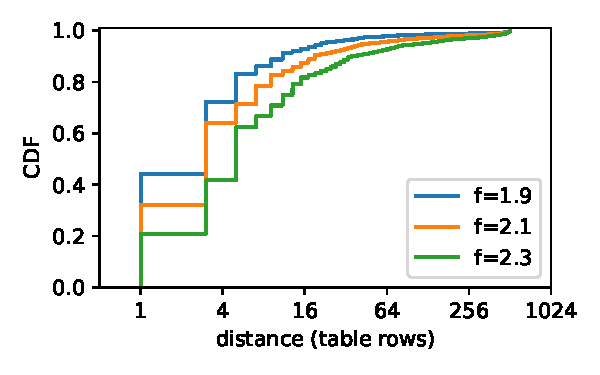
\includegraphics[width=0.99\linewidth]{fig/hash_factor.pdf}
        % \label{fig:hash_factor}
        % \caption{}
    \end{subfigure}
    \begin{subfigure}{0.3\linewidth}
        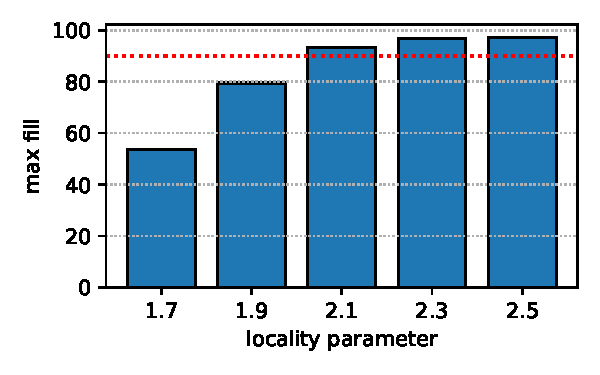
\includegraphics[width=0.99\linewidth]{fig/hash_fill.pdf}
        % \label{fig:hash_fill}
        % \caption{}
    \end{subfigure}.
    \vspace{-1em}
    \caption{
    \textbf{(a)} Dependent hashing for factor $f$.
    \textbf{(b)} CDF of distances between cuckoo locations dependent hashing on different exponential factors.
    \textbf{(c)} Exponential factor relation to max fill in cuckoo hash. 90\% fill marked in red.
    }
    \label{fig:locality-hashing}

\end{figure*}

Randomly spread cuckoo paths take many round trips to find
and lock. In this section we describe a novel
\textit{dependent} hashing algorithm which makes locality
between hash location a tuneable parameter. We describe the
tradeoffs of removing hash independence and demonstrate a
dramatic improvement in the round trips required to perform
insertions.

\begin{figure}[t]
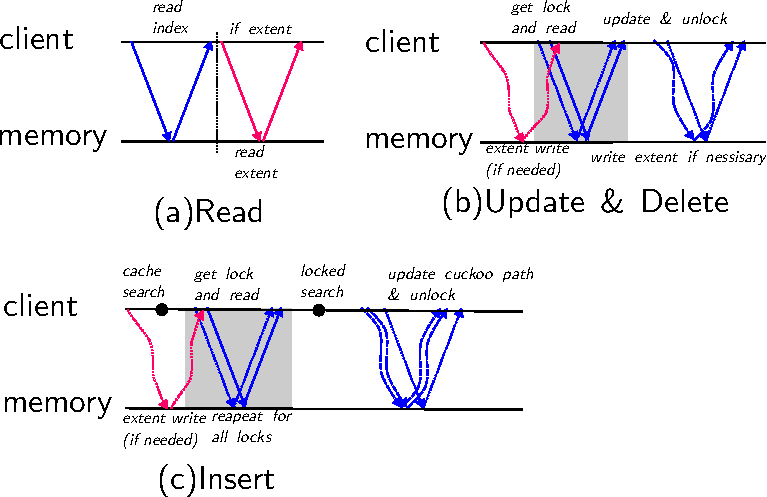
\includegraphics[width=0.99\linewidth]{fig/message_diagram.pdf}
%%
\caption{Rcuckoo's protocol for reads, inserts, deletes and
updates. Blue lines are index accesses, and red lines are
extent accesses. Solid lines are reads, dotted lines are
CAS, and curved dashed lines are writes.}
%%
\label{fig:message_diagram}
\end{figure}

\subsubsection{Dependent Hashing}

Our hashing algorithm borrows from both cuckoo and hopscotch
hashing to achieve tunable locality. The distance between
two hash locations is determined by probabilistically
\textit{dependent} rather than independent hash functions.
Locality between hash entries reduces the span of cuckoo
paths and increases the probability that multiple locks can
be set with a singe MCAS and both of a keys locations can be read
with a single RDMA message. However, high locality increases
the probability of hotspots in the table which decreases its
maximum fill factor.

Figure~\ref{fig:locality-hashing}(a) is our formula for
dependent hashing. The first hash location is chosen
uniformly at random, while second is chosen as an offset of
the first.  $f$ determines the max distance the second item
can be placed. Higher values of $f$ decrease locality.
Figure~\ref{fig:locality-hashing}(b) shows the distance
between hash locations as a CDF for different values of $f$.
Setting a constant bound on the distance between hash
locations leads to bad fill factors (on the order of
10-15\%). Our function places exponentially few locations
exponentially far apart using a third hash function $h_3(x)$
which generates a higher exponent at a logarithmic rate to
determine which locations will have large distances between
them\footnote{The value of $h_3(x)$ is the sum of trailing
zeros after calculating a keys 64bit hash value} These few,
but far apart hash locations increase the max fill by
alleviating hotspots in the table. While searching for
cuckoo paths with BFS these entries act as gateways for
paths to access less filled portions of the table. 

Figure~\ref{fig:locality-hashing}(c) shows how larger values of $f$
enable higher fill factors for tables with 100M entries. In
our experiments we use $f$ of 2.1 and an associativity of 8
as it provides a 90\% max fill an a 68\% probability that
hash locations are located 3 or fewer buckets apart.


\subsubsection{Locking}
\label{sec:locking}

\begin{figure*}[t]
    \centering
    \begin{subfigure}{0.3\linewidth}
        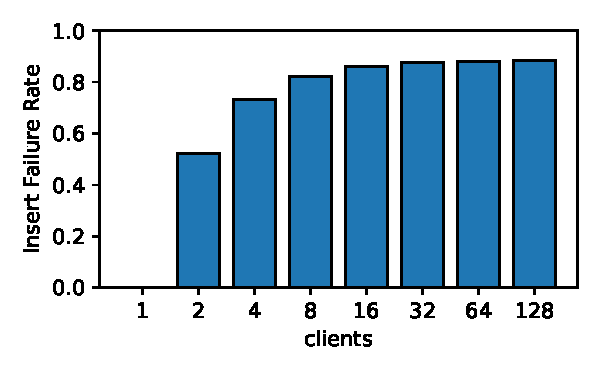
\includegraphics[width=0.99\linewidth]{fig/optimistic_failures.pdf}
        % \label{fig:optimistic_failures}
        % \caption{}
    \end{subfigure}
    \begin{subfigure}{0.3\linewidth}
        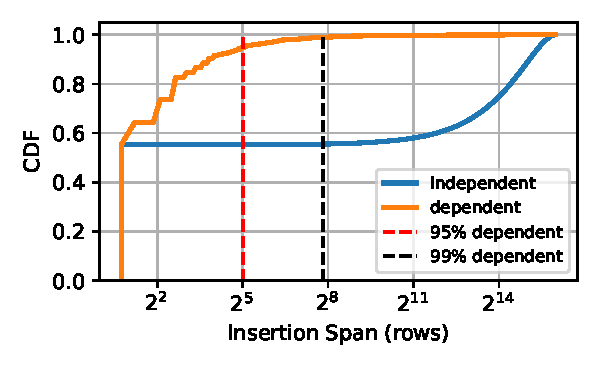
\includegraphics[width=0.99\linewidth]{fig/insertion_span.pdf}
        % \label{fig:insertion_span}
        % \caption{}
    \end{subfigure}
    \begin{subfigure}{0.3\linewidth}
        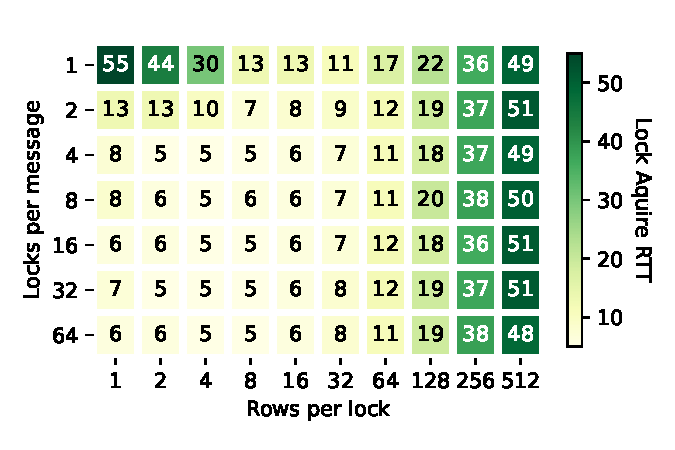
\includegraphics[width=0.99\linewidth]{fig/buckets_per_lock_vs_locks_per_message.pdf}
        % \label{fig:tbd}
        % \caption{}
    \end{subfigure}
    \vspace{-1em}
    \caption{
    \textbf{(a)} Failure rate of optimistic cuckoo insertions.
    \textbf{(b)} CDF of cuckoo spans for dependent and independent hashing. A cuckoo span is the distance between the smallest and largest index in a cuckoo path.
    \textbf{(c)} Round trips (99th percentile) on a table
    with 512 rows required per insert while filling a table
    to 95\%. 512 buckets per lock is a single global lock.}

    \label{fig:cuckoo-problems}

\end{figure*}

Increased path locality dually increases lock locality. If
multiple locks are within a 64 bit range of one another they
can be set atomically with a masked CAS.
Figure~\ref{fig:cuckoo-problems}(b) shows that 95\% of
dependent insertions span 32 or fewer rows while nearly 99\%
span 256 or fewer. If each lock protects 4 rows nearly 99\%
of insertions can have their locks acquired with a single
MCAS.

Figure~\ref{fig:cuckoo-problems}(c) shows the effect of lock
density (y-axis) and lock granularity (x-axis) on insert
performance. The top row shows the 99th percentile round
trips needed for inserts which aquire a single lock. In the
top left fine grained locking with one lock per message
results in 55 round trips. The far right colum shows how a
single global lock results in high contention. Dense tables
with a few rows per lock result in the fewest round trips.

% Using locks rather than opportunistic concurrency halves the
% latency of reads from two to one round trip. Opportunistic
% updates commit changes by atomically updating a pointer
% (with CAS) in the hash index to point to a new value. Both
% the index, then the value must be read for each operation.
% Values can not be inlined in the index as they are limited
% to the 64bit width of CAS. Rcuckoo uses locks to enable
% inlined entries which can be read in a single round trip.
% Locks introduce multiple challenges such as scalability,
% deadlocks and fault tolerance each of which is discussed
% below.

RCuckoo uses hardware NIC hardware features and lock
virtualization to achieve scalability, low contention and
high performance. The lock table is a linear array lock bits
and each bit locks one or more table rows. In our
experiments we use 16 rows per lock as it has a negligible
effect on contention and requires a single lock to be
acquired for vast majority of insertions.
%%
The lock table is located in NIC device memory which allows
atomic operations to scale linearly with reads and writes
and is 3x higher throughput on contented addresses than host
memory (see Figure~\ref{fig:rdma-benchmarks}). It is also
lower latency as operations to device memory avoid a PCIe
round trip.  Second, RDMA Masked Compare and Swaps (MCAS)
are used rather than CAS~\cite{rdma-masked-cas,sherman}. CAS
requires an exact 64 bit match to execute, while MCAS uses a
mask to only set the required bits. MCAS therefore reduces
contention while enabling locks to be as tightly packed.

Packing locks densely is important for reducing round trips
and because  NIC device memory is limited to 256KB which by
default limits table size. We use a \textit{virtual lock
table} to avoid limiting table size by device memory.
Multiple virtual locks map to a single physical lock. We use
modulo arithmetic to map virtual locks onto physical lock to
support arbitrarily large tables. Mapping multiple virtual
to a single physical lock leads to false sharing, clients
can be blocked unessisary on a lock.  In Section~\todo{TODO}
we show that on large lock tables the performance
degradation due to false sharing is low, and that lock
locality is maintained on virtual locks.

To avoid deadlock we aquire locks in incremental order.
Given a cuckoo path the rows are translated to virtual
locks, then to physical locks, then sorted. The sorted
locks are broken into 64 bit chunks which are mapped to
individual MCAS packets.  Lock requests are issued in order.
Clients continuously poll on lock requests and only move to
the next request only after the prior has been successfully
acquired.

Locality provides an additional opportunity to reduce round
trips by reading additional buckets. If locks are close
together but not contiguous clients issue a \textit{covering
read} spanning all rows between each bucket. We use 512
bytes as a max threshold. Covering reads synchronize a
clients cache for non-locked rows. If the second search
fails to find a valid cuckoo path the next iterations
speculative search will benefit from the fresh read.
Figure~\ref{fig:table-diagram} illustrates a covering read
between keys $K$ and $C$.

% Speculative locks may not be sufficient to complete an
% insertion.  However, due to locality hashing there is a high
% probability that a valid path does exist in the neighborhood
% of the speculative locks. 
% If two speculatively locked rows
% are close enough together clients issus a single
% \textit{covering read} spanning both rows. Covering reads
% populate a clients cache and dramatically increase the
% probability that if the first speculative search fails, a
% subsequent search will succeed.  We set the max threshold
% for covering reads to 512 bytes in all our experiments.
% Figure~\ref{fig:table-diagram} illustrates an insertion of
% key $K$ displacing key $C$. Here the speculative search
% marked the rows for $C$ and $K$ to be locked. A covering
% read (red) spans the rows between both entries.

Clients may fail while holding locks leaving them set and
stranded. Clients detect failed locks by timing out on them
while acquiring them. To separate failures from clients
acquiring a long list of contended locks clients are given a
bounded time to aquire their locks. If a client takes longer
than this time to aquire all of its locks it releases all
held locks and starts the process again to prevent false
failure detection. Our complete fault detection and recovery
mechanism is described in Section~\ref{sec:fault-tolerance}.

\subsection{Fault Tolerance}
\label{sec:fault-tolerance}

The table must be repaired if a client fails while holding a
lock. In our fault recovery algorithm non-failed clients
aquire repair leases to reclaim the locks of failed clients
and then perform the operations required to return the table
to a valid state. In this section we describe how RCuckoo
clients detect faults, repair the table, and prevent stray
RDMA writes from failed clients from corrupting the table.

\subsubsection{Failure Detection} 
\todo{note that we don't know who has the lock or when they got it}

Clients detect failures with timeouts triggered when a lock
acquisition or read fails repeatedly and the state of the
locked or read rows is unaltered by other clients.  True
failures are distinguished from frequently accessed rows by
checking CRCs which are modified on every row update due to
row version numbers (Section~\ref{sec:table-design}).
Clients reset their failure timers whenever a CRC changes
between requests.


\todo{talk about the actual timeout value} We view failures
as a rare but essential component of our protocol. As such
our fault timers are set conservativly. Failure timers for
locks must include locking time, second search time, and
update transit time. We bound locking time (Section
~\ref{sec:locking}), search, and message propagation is
measured in single digit microseconds. We additionally want
to ensure that network conditions are not causing continual
RDMA retries. We set the max RDMA operation retry number to
3 for all our experiments. We set our failure timeout to
100ms as it is orders of magnitude above our 99th percentile
insert time (50us) and above the RDMA retry limit.


\subsubsection{Repair Leases}
\todo{mention repair lease table}

Repair leases provide clients with exclusive permission to
reclaim locks on a region of the table. The table is broken
into $n$ regions so repairs can be executed in parallel (see
Figure~\ref{fig:table-diagram}). Leases are set with 64 bit
CAS and track the lease holders QP id, a set bit, and a
counter (incremented on each acquisition).  Failures while
holding a lease are easier to detect than normal locks as a
leases owner and liveness are tracked within it.  Leases are
revoked using a similar timeout to normal locks. When a
client times out on a lease it claims it for itself and
marks the lease holder as failed (see
Section~\ref{sec:stale-writes}).  A lock is reclaimed once a
client both times out on a lock and acquires the locks
repair lease. 


\subsubsection{Table Repair} 
\label{sec:table-repair}

Cuckoo updates occur along a path
and client failures could occur at any point along an
insertion path. Updates and Deletes are a special case where
the path length is 1. If a client fails mid modification it
can leave the table in 3 distinct states based on where in
the update it fails. 

Our table design ensures that clients can perform repairs
and recover from all states a failed client may have
created. Recovery is simple if a client with locks fails
prior to issuing its updates or if it fails before releasing
its locks. A client with a repair lease can simply set
unlock the stranded lock in this case. Failures during
modifications require special care to recover from. All
modification operations Update, Delete, and Insert write new
entries as a cuckoo path~\footnote{updates and deletes are a
cuckoo path of length 1}. As described in
Section~\ref{sec:insert} cuckoo paths are executed by first
setting an open entry to claim it and migrating entries
backwards along the path until a new entry is written. If
partially executed this algorithm can produce 3 distinct
states.

\begin{enumerate}
    \item{A duplicate entry exists and one has a bad CRC}
    \item{A duplicate entry exists and both have correct CRCs} 
    \item{No duplicate exists but one row has a bad CRC}
\end{enumerate}

To repair the table a client first detects which state the
table is in and then transitions the table forward through
the states with a deterministic sequence of operations so
that failures during recovery can be continued by any other
client. A client detects the state issuing reads to all rows
protected by the stranded lock. Then all entries within the
rows have both hash locations read individually to check for
duplicates. The error state can be detected by the presence
of duplicates in these rows and the existence of bad CRCs.

Table corrections are issued as a batched sequence of 3 or
fewer writes as follow: $1 \rightarrow 2$ - write a new CRC
for the bad duplicate.  $2->3$ - Set the duplicate in the
second hash location to empty. $3\rightarrow$ - recalculate
and write a new CRC. After a client has issued its repair
sequence it unlocks the reclaimed lock and returns its
lease.


\subsubsection{Preventing Stale Writes}
%%
\label{sec:stale-writes}
%%

An RDMA connection must be closed, transitioned to an error
state, or have it's permissions revoked to prevent its
operations from being executed on memory. Because we assume
remote memory is passive (it will not tear down connections)
and that faulty clients will not tear down their connections
it is possible that the connection of a failed client will
stay open and stale writes may be delivered to memory after
a faulty clients lock is revoked. We use conservative
timeouts to out-wait network delays and RDMA retransmissions
at the cost of recovery latency. 

At the time of writing the infiniband specification does not
enable clients to modify each others permissions. Type II
memory windows enable clients to remove their own
permissions using the \textit{send with invalidate} verb. If
the specification were extended to allow a client with
elevated privileges to revoke the permissions of a faulty
client it would provide a clean means of handling client
failure in the disaggregated setting. Given the current
specification a client can corrupt the QP's of another by
sending a crafting an invalid packet and sending to their
queue pair pair~\cite{redmark}[attack 2]. For this attack to
work the packet sequence number of the shutdown packet must
match the sequence number of the receiver so $2^{24}$
packets must be sent to ensure a connection is corrupted
successfully.
